\chapter{Resultados e discussão}
\label{cap:resultados}

Apresente os resultados de forma organizada e discuta sua relação com os
objetivos e com a literatura. Não substitua a análise por uma sequência de
figuras ou tabelas: explique o que cada resultado mostra e quais são suas
limitações.

\section{Espectro de energia}

Para o oscilador harmônico quântico, os níveis de energia são
\begin{equation}
  E_n = \hbar\omega\left(n+\frac{1}{2}\right),
  \qquad n=0,1,2,\ldots.
  \label{eq:energia}
\end{equation}
Em particular, o estado fundamental possui energia não nula,
\(E_0=\hbar\omega/2\).

\begin{table}[htbp]
  \centering
  \caption{Primeiros níveis de energia do oscilador harmônico}
  \label{tab:niveis}
  \begin{tabular}{cccc}
    \toprule
    \(n\) & \(E_n\) & Paridade & Nós \\
    \midrule
    \niveisTabela
    \bottomrule
  \end{tabular}
  \fonte{Elaboração própria; dados calculados em \texttt{lua/conteudo.lua}
  para \(\hbar\omega=\qty{250}{\milli\electronvolt}\).}
\end{table}

\begin{frame}{Funções de onda}
  \framesubtitle{Soluções normalizadas sobre o potencial parabólico}
  \begin{columns}[T,onlytextwidth]
    \begin{column}{0.35\textwidth}
      \begin{destaque}{Forma geral}
        \[
          \psi_n(\xi) = N_n\,H_n(\xi)\,e^{-\xi^2/2}
        \]
        {\scriptsize\color{fisicamuted}%
         $N_n=(2^n n!\sqrt{\pi})^{-1/2}$,\quad
         $\xi=\sqrt{m\omega/\hbar}\,x$}
      \end{destaque}
      \begin{itemize}
        \item $n$ nós e paridade $(-1)^n$
        \item $|\psi_n|^2$: densidade de probabilidade
      \end{itemize}
    \end{column}
    \begin{column}{0.62\textwidth}
      \centering
      \begin{tikzpicture}
        \begin{axis}[
          width=\linewidth,
          height=5.55cm,
          axis lines=left,
          axis line style={draw=fisicamuted,line width=0.5pt},
          xmin=-4.1, xmax=4.1,
          ymin=0, ymax=5.7,
          xlabel={$x\,/\,\sqrt{\hbar/m\omega}$},
          ylabel={$E\,/\,\hbar\omega$},
          xlabel style={font=\scriptsize,text=fisicamuted},
          ylabel style={font=\scriptsize,text=fisicamuted},
          tick label style={font=\scriptsize,text=fisicamuted},
          grid=major,
          grid style={draw=fisicamuted!12},
          legend style={
            at={(0.03,0.97)},anchor=north west,
            draw=none,fill=fisicabg,fill opacity=0.85,text opacity=1,
            text=fisicafg,font=\scriptsize,row sep=0pt},
          legend cell align=left,
        ]
          \plotOscilador
        \end{axis}
      \end{tikzpicture}
    \end{column}
  \end{columns}
\end{frame}


\begin{figure}[htbp]
  \centering
  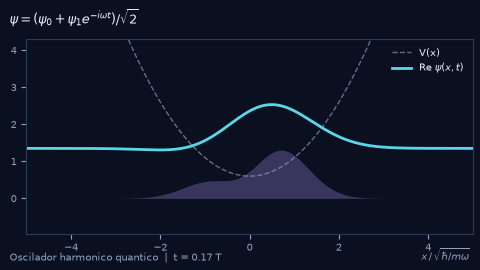
\includegraphics[width=0.8\textwidth]{videos/demo-oscilador.png}
  \caption{Visualização de uma superposição de estados do oscilador
  harmônico quântico}
  \label{fig:exemplo}
  \fonte{Material de demonstração incluído no repositório.}
\end{figure}
